\documentclass[10pt,a4paper]{article}

\usepackage[margin=2cm]{geometry}
\usepackage[T1]{fontenc}
\usepackage{lmodern}
\usepackage{microtype}
\usepackage{booktabs}
\usepackage{array}
\usepackage{float}
\usepackage{graphicx}
\usepackage{xcolor}
\usepackage{enumitem}
\usepackage[hidelinks]{hyperref}
\graphicspath{{../outputs/figures/}}
\setlist{nosep, leftmargin=*}
\setlength{\parskip}{3pt}
\setlength{\parindent}{0pt}
\setlength{\emergencystretch}{2em}

\title{\vspace{-1.2cm}RAG Assignment: Baseline vs.\ Re-Ranking}
\author{Shreyas Deb}
\date{October 2026}

\begin{document}
\maketitle
\begin{center}
\textbf{Code:} \url{https://github.com/shrey715/shiori} \quad
\textbf{Document:} ICC Men's T20 World Cup 2026 Playing Conditions (106 pages)
\end{center}

\section*{Setup}

\begin{itemize}
  \item \textbf{Document.} I picked the ICC T20 World Cup 2026 playing conditions because they are full of ``unless / except / shall not'' clauses, and the appendices (DRS, Super Over, warm-up matches, reserve day) override the main rules. The PDF is from February 2026, so the LLM can't have seen it.
  \item \textbf{Chunking.} I split by clause number (e.g.\ 9.1, 9.1.1), merged consecutive clauses of the same section up to $\sim$180 tokens, and dropped headers, diagram labels and blank forms. That gave \textbf{440 chunks}. I kept them small on purpose: with big chunks the answer is almost always in the top 3 already. Every chunk exists as \textbf{A} (plain text) and \textbf{B} (section title + text).
  \item \textbf{Models.} Bi-encoders: \texttt{all-MiniLM-L6-v2} and \texttt{bge-small-en-v1.5} (FAISS, exact cosine). Re-rankers: \texttt{ms-marco-MiniLM-L6-v2} (used for Answer 2) and \texttt{bge-reranker-base} (rankings only). LLM: \texttt{Qwen3-32B-AWQ} on vLLM over 4$\times$RTX 2080 Ti, temperature 0.
  \item \textbf{Questions.} 40 questions in 4 tiers of 10, each harder than the last: direct wording, fan paraphrase, exceptions/negations, and traps/cross-references. Each has a gold chunk and an expected answer, checked against the rule text.
  \item \textbf{Grading.} Every answer (No RAG, Answer 1, Answer 2) was graded against the expected answer as correct (1), partial (0.5), wrong or abstain (0), by the same LLM with a fixed rubric. A blind second grader (Claude Haiku) agreed exactly on 79\% and within one step on 97\%. I fixed the 5 clear grader errors by hand.
\end{itemize}

\section{Bi-encoder vs.\ Cross-encoder}

A \textbf{bi-encoder} encodes the question and each chunk \emph{separately} into one vector each, and relevance is just their cosine similarity. Chunk vectors don't depend on the question, so I compute them once, store them in FAISS, and a search is one dot product per chunk. The catch is that the whole chunk gets squashed into a single vector before the question even exists, so it mostly captures topic and word overlap. ``can'' vs.\ ``cannot'', or a rule vs.\ its exception, end up very close in that space.

A \textbf{cross-encoder} takes the question and a chunk \emph{together} as one input, so every question token attends to every chunk token, and it outputs one relevance score. It can check whether the chunk actually answers \emph{this} question (the right condition, the right exception, the right match type). It's much more accurate, but nothing can be precomputed: every (question, chunk) pair needs a full forward pass. That's why it's only used to re-rank the bi-encoder's top 10.

\section{Qualitative \& Rank Shift Analysis}

\subsection{Overall}
Re-ranking improved MRR in all 4 setups and hit@3 in 3 of 4 (Table~\ref{tab:ret}). Over all setups it moved the gold chunk from rank 4--10 into the top 3 in \textbf{16 cases}, and pushed it out of the top 3 in 9. 15 of the 16 fixes are in tiers 3--4; tier 1 was already 100\%.

The bigger \texttt{bge-reranker-base} (278M params) was about the same as the 22M \texttt{ms-marco} one, so a bigger re-ranker didn't buy much here. Adding section titles to chunks (B) didn't help consistently either.

\begin{table}[H]
\centering\small
\begin{tabular}{lcccc}
\toprule
setup & hit@3 base $\to$ re-ranked & MRR@10 base $\to$ re-ranked & answer score A1 $\to$ A2 \\
\midrule
MiniLM, plain (A)  & 0.65 $\to$ 0.70 & 0.53 $\to$ 0.65 & 0.68 $\to$ 0.65 \\
MiniLM, titled (B) & 0.62 $\to$ 0.68 & 0.50 $\to$ 0.65 & 0.59 $\to$ 0.64 \\
bge, plain (A)     & 0.70 $\to$ 0.78 & 0.63 $\to$ 0.69 & 0.65 $\to$ 0.72 \\
bge, titled (B)    & 0.75 $\to$ 0.75 & 0.60 $\to$ 0.69 & 0.70 $\to$ 0.72 \\
\bottomrule
\end{tabular}
\caption{Retrieval and answer quality before and after re-ranking with \texttt{ms-marco} (40 questions).}
\label{tab:ret}
\end{table}


\subsection{Failure cases fixed by re-ranking}
In every case below the important chunk sat outside the top 3, so the LLM in Pipeline 1 never saw it.

\begin{table}[H]
\centering\small
\newcolumntype{L}[1]{>{\raggedright\arraybackslash}p{#1}}
\begin{tabular}{L{3.0cm}L{1.7cm}L{1.8cm}L{4.1cm}L{4.1cm}}
\toprule
question & type & gold chunk & Answer 1 (baseline) & Answer 2 (re-ranked) \\
\midrule
q23: can a concussed player be replaced by someone not on the list? & exception & c008 (1.2.7.1.3.4) \textbf{\#9 $\to$ \#3} & ``No, a concussed player can only be replaced by a player who is on the nominated list.'' \textbf{Omits the exception.} & ``Yes, \ldots{} but only under exceptional circumstances. \ldots{} the ICC Match Referee will consider the request.'' Correct. \\
q35: 7-over rain game, max overs per bowler? & buried chunk & c091 (13.9.2.2) \textbf{\#4 $\to$ \#1} & ``1 over \ldots{} no bowler may bowl more than one-fifth'' (the rule for 10+ overs). \textbf{Misstates the rule.} & ``2 overs, as per rule 13.9.2.2.'' Correct. \\
q28: can the non-striker sneak a run during the run-up? & negation & c314 (41.16) \textbf{\#5 $\to$ \#2} & ``Not in the context.'' (top 3 were the wrong run-out clauses) & ``No \ldots{} Dead ball, \ldots{} disallow the attempted run, and award 5 Penalty runs.'' Correct. \\
q36: start time of the final on the reserve day? & keyword trap & c069 (12.7.1) \textbf{\#4 $\to$ \#2} & ``The final will start \ldots{} when the coin toss takes place'', no time given. \textbf{Made up.} & ``The final starts at 19:00.'' Correct. \\
q38: free hit called wide, can he be stumped? & exception over 2 chunks & c175 \#4 $\to$ \#3, c174 \#6 $\to$ \#2 & ``Yes, \ldots{} the batter can be out stumped.'' \textbf{Wrong:} uses the general wide rule. & ``No, \ldots{} only \ldots{} the circumstances that apply for a No ball, even if \ldots{} called Wide.'' Correct. \\
\bottomrule
\end{tabular}
\caption{Showcase failures (setups: q23, q35 MiniLM-A; q28 MiniLM-B; q36, q38 bge-A).}
\end{table}

\begin{figure}[H]
\centering
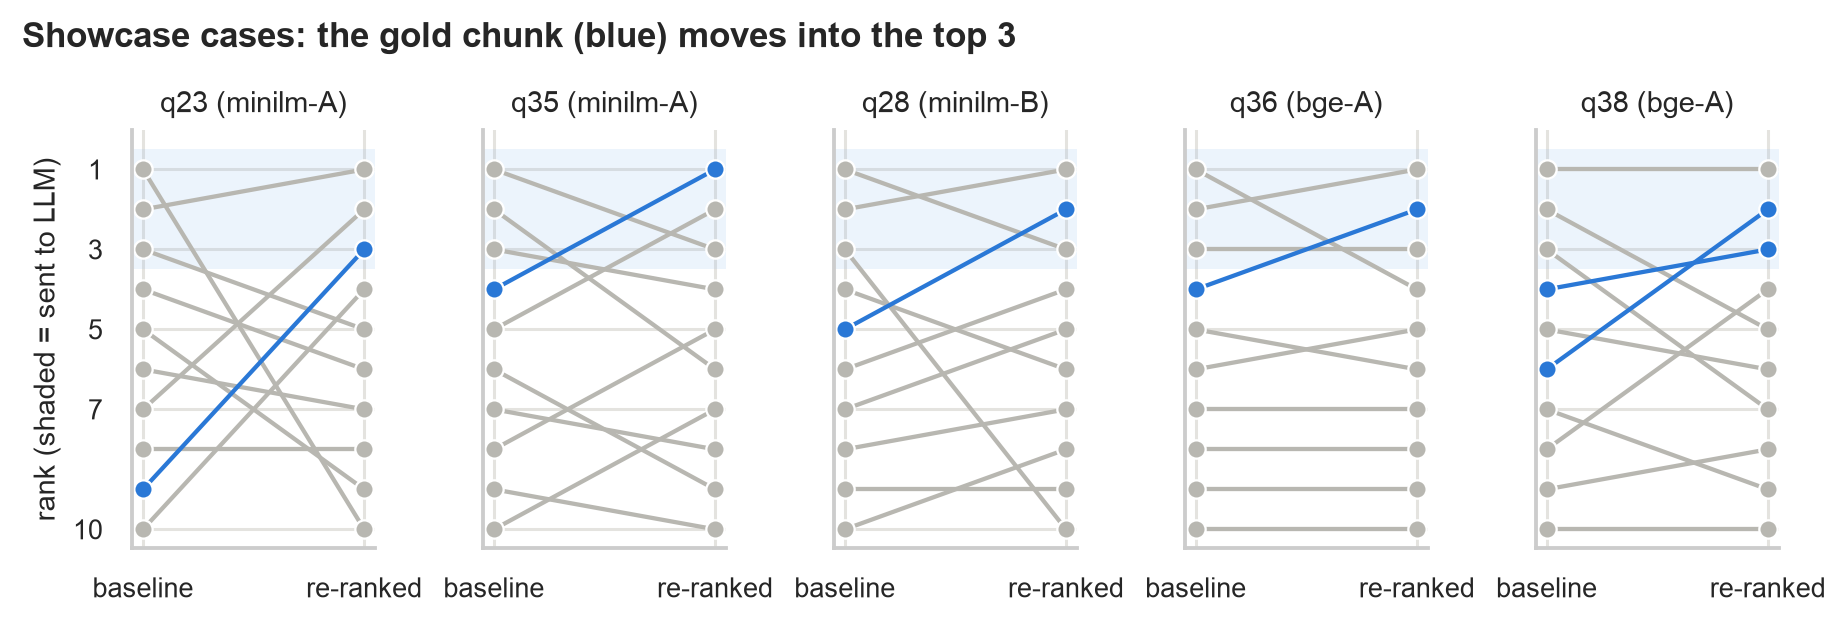
\includegraphics[width=0.95\linewidth]{showcase_bump.png}
\caption{Rank of each top-10 chunk before and after re-ranking for the cases above; gold in blue, shaded = top 3 sent to the LLM.}
\end{figure}

So the baseline failed in exactly the ways the assignment describes: it \textbf{left out an exception} (q23, q38), \textbf{applied the wrong rule} (q35), \textbf{made something up} (q36), or gave up because the right clause wasn't there (q28). In 12 of the 16 rank fixes the answer improved too.

\subsection{Where re-ranking failed}
\begin{itemize}
  \item \textbf{Regressions.} The cross-encoder can also be fooled by surface matches. For q22 (``umpire calls a wide, keeper whips the bails off'') it ranked helmet and fielder clauses first, pushing the right one (22.9) from \#2 to \#5, and the answer went from correct to wrong. For q33 (``can the same bowler bowl the next Super Over?'') a clause about the ``same bowler'' offending a third time (41.13.4) beat the Super Over rule (\#3 $\to$ \#7).
  \item \textbf{Lost chunks.} For 5 questions the gold chunk was below rank 10 in every setup, so the re-ranker never saw it. E.g.\ for ``Is there a follow-on in T20?'' the chunk just says ``Shall not apply.'' and shares no words with the question.
  \item \textbf{Reading failures.} For q24, q31 and q40 the gold chunk was \#1 and the answer was still wrong: the LLM read ``However, \ldots{} they shall refuse'' as the rule (q24), ``complete or replay'' as ``replay'' (q40), and ignored ``no more than 11 may bat'' (q31). Retrieval can't fix that.
\end{itemize}

\subsection{Is it just the LLM's own knowledge?}
No. Without the document the LLM is \textbf{wrong 55\% of the time} and almost never says it doesn't know. Splitting the questions into general cricket law vs.\ tournament-specific rules makes it clear (Figure~\ref{fig:scope}): the model knows general laws (0.53) but not this tournament's rules (0.20). On those, RAG takes it to 0.64, and re-ranking to \textbf{0.73}. On general laws re-ranking slightly hurt (0.67 $\to$ 0.63), mostly because of the q22 regression.

\begin{figure}[H]
\centering
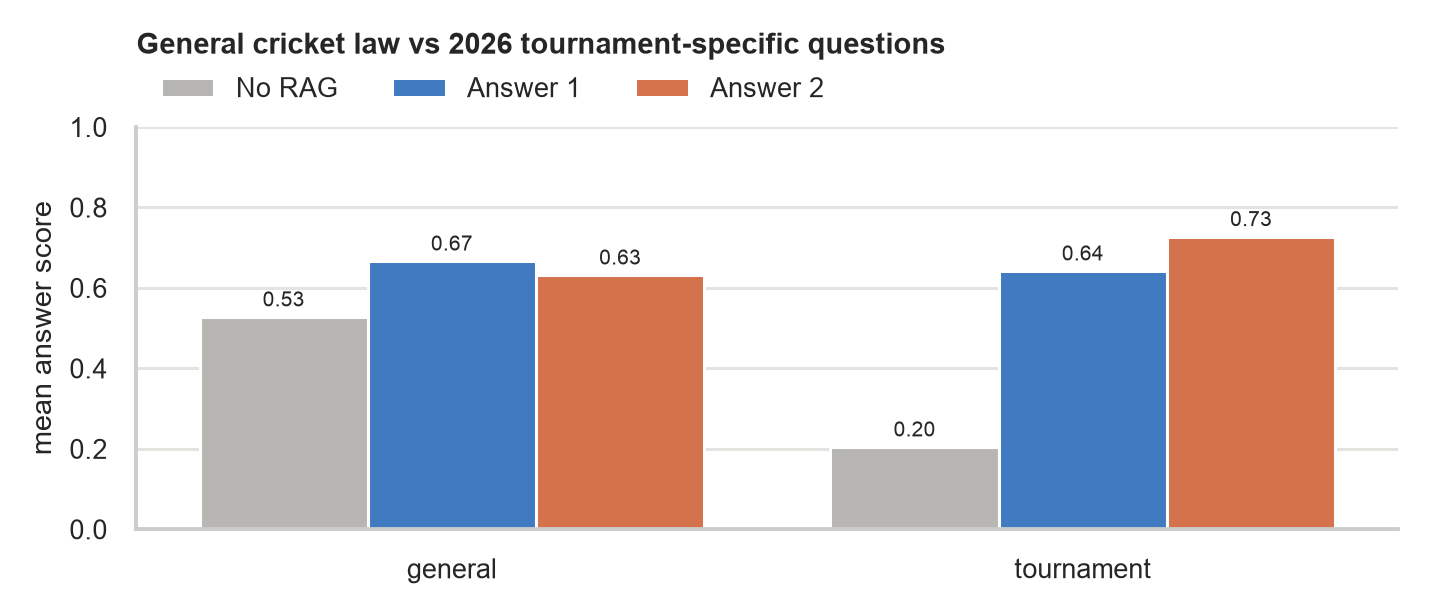
\includegraphics[width=0.55\linewidth]{scope_scores.png}
\caption{Mean answer score by question type and mode.}
\label{fig:scope}
\end{figure}

\section{Latency Profiling}

All on one RTX 2080 Ti (MiniLM + \texttt{ms-marco}), mean over 40 queries after 5 warm-ups, with \texttt{cuda.synchronize()} around each call.

\begin{table}[H]
\centering\small
\begin{tabular}{lr}
\toprule
stage & ms / query \\
\midrule
query embedding & 6.0 \\
FAISS search (top 10) & 0.05 \\
cross-encoder on 10 pairs & 14.2 \\
\midrule
\textbf{Pipeline 1 (baseline retrieval)} & \textbf{6.2} \\
\textbf{Pipeline 2 (retrieval + re-ranking)} & \textbf{19.8} \\
\midrule
cross-encoder on all 440 chunks & 295 \\
Pipeline 2, 40 queries batched & 7.3 \\
\bottomrule
\end{tabular}
\caption{Retrieval latency per query on GPU.}
\end{table}

Re-ranking adds about \textbf{14 ms per query (3.2$\times$)}, almost all of it the cross-encoder; the FAISS search itself is basically free. In absolute terms that's cheap, and small next to the LLM call (seconds), so for these accuracy gains it's clearly worth it. Batching queries brings Pipeline 2 down to 7 ms each.

\section{Scaling: why not cross-encode everything?}

Because the cost grows with the number of chunks, and nothing can be precomputed. A cross-encoder needs the question, so for every new query it has to run one forward pass per chunk. Here, scoring all 440 chunks took \textbf{295 ms per query}, about 6{,}000$\times$ slower than the FAISS search (0.05 ms). That's $\sim$0.67 ms per chunk, so a collection of 1M chunks would take about \textbf{11 minutes per query} on this GPU. Bi-encoder chunk embeddings are computed once, offline, and vector search (especially approximate indexes) stays in milliseconds even for millions of chunks.

So the two-stage setup gets most of the benefit for a fraction of the cost: the cheap bi-encoder narrows millions of chunks to 10, and the expensive cross-encoder only has to sort those 10. The trade-off, which my lost cases show, is that re-ranking can only fix what the first stage retrieves. A chunk that the bi-encoder ranks 100th stays lost.

\end{document}
